% ==============================================================================
% 尾声：继续前行 (Epilogue: Moving On)
% ==============================================================================

\chapter*{尾声：继续前行}
\addcontentsline{toc}{chapter}{尾声：继续前行}
\markboth{尾声：继续前行}{尾声：继续前行}
\label{sec:epilogue}

\begin{center}
  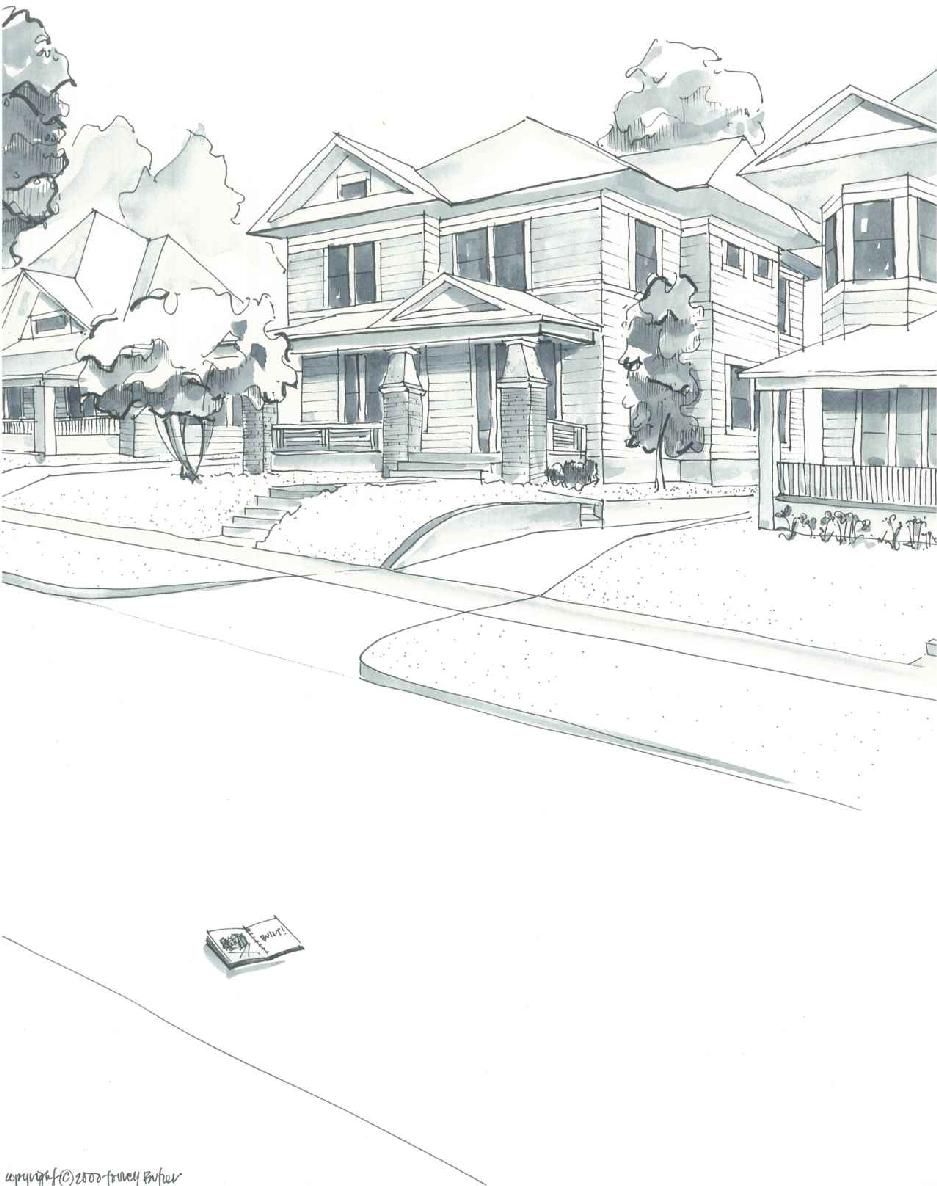
\includegraphics[width=0.7\textwidth]{images/00784.jpeg}
\end{center}

至此，你已经走完了这部关于计算与编程——或者如我们一直强调的，\textbf{程序设计}（program design）——的引论之旅。尽管在这两个广袤的学科领域中还有太多激动人心的知识等待你去探索，但此刻正是一个极佳的停驻点，让我们静下心来回顾、凝练并展望未来。

\section*{计算 (Computing)}
\addcontentsline{toc}{section}{计算 (Computing)}
\label{sec:epilogue_computing}

在小学时代，你学会了用数字进行基础运算。起初，你用数字来清点现实世界中的具体事物：3 个苹果、5 位好友、12 个面包圈。不久之后，你接触到了加、减、乘、除四则运算，接着又认识了分数。最终，你步入了变量与函数的殿堂，老师们将其称之为代数。在代数的世界里，变量指代数字，而函数建立了数字到数字之间的对应关系。

因为在整个受教育过程中你始终与数字打交道，你可能从未深入思考过：\textbf{数字本质上只是一种用以表征现实世界信息的手段}。是的，你最初是从三只小熊、五匹饿狼和十二匹骏马开始的；但到了高中，再也没有人刻意提醒你这种符号与现实之间的映照关系了。

当你从纯粹的数学演算跨入计算机科学时，\textbf{从现实信息（Information）到计算数据（Data）的双向映射跃迁便成为了最核心的命题}。如今的现代程序每天都在处理对音乐、视频、微观分子、化合物、商业案例分析、电路拓扑图以及工程蓝图的数字化表征。幸运的是，你根本不需要将所有这些五彩斑斓的现实信息全部强行编码为冷冰冰的数字，更不必退化到苦不堪言的 0 和 1；如果非得那样做，编程生活将变得枯燥乏味到难以想象。相反，计算科学彻底推广了算术与代数的内涵，使得当你编写程序时，能够自然、直接地使用字符串、布尔值、字符、结构体、列表、树乃至作为一等公民的函数等极其丰富的数据类型进行思考与编码。

每一类数据及其操作函数都伴随着严密的\term{等式定律}（equational laws）来阐释其内在含义，正如数字与代数函数所遵循的运算法则一样。尽管诸如 \code{(+ 1 1)} 求值为 2 以及 \code{(not \#true)} 等于 \code{\#false} 这样的基本等式极其质朴，但你完全可以凭借它们精确预测极其庞大复杂的完整程序的运行时行为。当你运行一个程序时，本质上只是在调用它的某个顶层函数；这一动作完全可以通过我们在插曲 1 中首次介绍的 $\beta$ 归约规则（beta rule）予以形式化解释：一旦形参被实参替换，相应的数据计算定律便立即接管接力棒展开代数化简，直至最终化为一个不可再约简的值，或化为下一个函数应用。

是的，这便是整个计算世界的根本基石。

\section*{程序设计 (Program Design)}
\addcontentsline{toc}{section}{程序设计 (Program Design)}
\label{sec:epilogue_design}

一个典型的现代软件工程项目往往需要成百上千名程序员的通力协作，其最终产物通常由成千上万个相互协作的函数组成。在这样一个大型项目的完整生命周期中，开发人员总是在不断地更迭交替。因此，\textbf{程序的体系结构与设计结构，本质上是程序员之间跨越时空进行思想沟通的核心媒介}。当你面对一段前人在数月甚至数年前写就的代码时，程序本身必须能够清晰地自白其设计目的及其与其他组件之间的依存关系——因为当初写下这行代码的原作者很可能早就离开团队了。

在如此高度动态演进的工程环境中，程序员唯有秉持极其严谨自律的工程纪律来构建程序，才有可能在保证合理工作时长的前提下，持续交付出高质量、高可靠的软件产品。严格遵循系统化的设计方法，能够从根本上保证程序的组织架构具备极佳的可理解性。唯有如此，后来的协作者才能从容看清局部组件与系统全局，从而迅速定位并修复 Bug，或敏捷添加全新的业务功能特性。

本书所倾囊相授的\term{程序设计配方}（Design Recipe），正是这样一套经过千锤百炼的系统化方法学。只要你在编写任何自己真正在乎的程序，就应当始终如一地践行它：
\begin{enumerate}
  \item 你从对信息世界的深入剖析以及对表征该信息的数据定义（Data Definitions）启程；
  \item 随后制定周密的函数心愿单（Work List）；
  \item 若需求规模庞大，你采用敏捷迭代的方式精细演进：首先提炼出一个最小功能子集，迅速交付出一个用户或客户能够上手交互的可用原型；通过观察用户的实际交互反馈，你将极其敏锐地洞察到心愿单上下一个最应当攻克的优先级组件。
\end{enumerate}

设计一个大型程序（乃至设计哪怕一个最微小的函数），都必须对其计算目标建立严谨透彻的理解。除非你能用一句凝练准确的\term{目的说明}（Purpose Statement）清晰勾勒出一段代码的存在价值，否则你绝不可能为未来的协作者产出任何有价值的遗产。精心构造丰富的功能示例，并将其转化为一整套自动化\term{单元测试套件}（Test Suite）。这套测试套件在软件后续漫长的维护重构中具有无可估量的价值——任何对代码进行修改的人，都能立即重跑测试，秒级重获“底层核心逻辑依然完好无损”的确定性与安全感。

在软件生命周期的某个时刻，程序终归会出现故障。其他开发者可能会以未曾预料的方式调用你的模块，真实用户可能会在实际体验中发现与预期不符的偏差。正是因为你从第一天起就以高度系统化的方式设计了代码，面对 Bug 时你将成竹在胸、临危不乱：
\begin{enumerate}
  \item 首先为顶层主函数编写一个能够稳定复现 Bug 的\textbf{失败测试用例}；
  \item 沿着调用链路，自顶向下为主函数涉及的每个子函数衍生对应的测试用例；
  \item 那些依然顺利通过测试的函数便排除了嫌疑；而未通过测试的函数必然就是 Bug 的温床（有时是几个有缺陷的函数相互串通引发了异常）；
  \item 若该出故障的函数复合了其他底层组件，继续向下细化测试；否则，你已经成功将 Bug 精准捕获在掌心！
  \item 当你修复缺陷并看到整个系统重新全绿通过全部测试套件时，你确凿无疑地知晓：问题已经被彻底搞定！
\end{enumerate}

无论你之前多么辛勤，\textbf{一个函数或程序在第一次全部通过测试套件时，绝对不意味着设计工作的结束}。你必须留出专门的时间来审查代码的设计坏味道（design flaws）与重复模式。一旦发现任何重复出现的结构模式，务必运用抽象提炼出更高阶的通用函数，实现软件架构中神圣的\term{单点控制原则}（Single Point of Control）。

只要你恪守这些工程准则，你便能以合理的精力投入，持续产出坚如磐石的软件工程杰作。你的程序之所以能够优雅稳定地运转，是因为你从数学底层透彻洞悉了它为何能够运转、如何运转。其他需要修改或扩展你系统的人也能够秒懂你的意图，因为你的代码在字里行间清晰地诉说着它的思考过程与崇高目的。

读完本书，你已经迈出了坚实的第一步。现在，轮到你踏上\textbf{练习、练习、再练习}的征途了。关于程序设计与计算科学，还有无比宽广的星辰大海等待你在未来的求索中去遨游！

\section*{向前看，致开发者与计算机科学家}
\addcontentsline{toc}{section}{向前看，致开发者与计算机科学家}
\label{sec:epilogue_cs}

此刻的你或许正在思考：下一步究竟该学习什么？答案是双向并进：\textbf{研习更高级的程序设计，并探索更深邃的计算科学}。

作为一名志存高远的程序设计学子，你的下一个核心任务是：学习如何将本书学到的系统化设计配方无缝迁移并应用到工业级全功能编程语言中。其中一些语言与本书所用的教学语言血脉相通（例如完整的 Racket、Clojure、OCaml、Haskell），过渡过程将行云流水；而另一些语言（如 Java、TypeScript、C++、Rust、Go）则需要你转换思维视角，因为它们提供了形式化的静态类型系统（Types）以及面向对象类与结构封装（Classes \& Objects），能够在程序运行之前就通过编译器交叉检查函数签名与数据约束。

此外，你还需要学习如何将设计配方扩展至现代工程\term{组件}（Components）与\term{开发框架}（Frameworks / “Stacks”）的构建与使用中。通俗地说，各类软件框架高度抽象了现代系统通用的通用基础能力——例如图形用户界面（GUI）、分布式网络通信、持久化数据库连接以及 Web 全栈架构。你必须学会实例化这些高级抽象，并在程序中将其优雅编排复合为有机协调的大型系统。

\begin{notebox}[课外探索推荐]
凭借你在本书中筑牢的扎实功底，学习本书教学语言背后的工业级母体语言——Racket，将是一段极其轻松愉悦的旅程。推荐阅读《Realm of Racket》，开启探索更浩瀚 Racket 生态的奇妙冒险！
\end{notebox}

作为一名计算科学的探求者，你还必须极大拓展自己对计算过程物理与工程本质的理解深度。本书重点聚焦于描述计算过程本身的代数定律；而要成长为一名真正的软件工程师，你必须在理论与工程实践两个层面上深刻理解计算所付出的\textbf{代价}。深入研读算法渐近复杂度（$\mathcal{O}$ 记号）是迈向这一方向的坚实起点；而学会运用性能剖析器（Profiler）对实际软件进行性能测量与瓶颈分析则是日常研发中的核心刚需。在此之上，你还需要深入计算机硬件底层结构、操作系统分层、网络协议栈以及各个垂直应用领域中的专门算法。

\section*{向前看，致会计师、记者、外科医生及所有人}
\addcontentsline{toc}{section}{向前看，致会计师、记者、外科医生及所有人}
\label{sec:epilogue_everyone}

你们当中的一部分读者当初翻开此书，或许只是出于好奇，想看一看所谓“计算”与“编程”究竟是怎么一回事。现在的你已经懂得：计算绝非高深莫测的黑魔法，它本质上只是日常算术运算的高度哲学化推广；你也切身体会到了系统化程序设计思维蕴藏的巨大威力。即便你未来再也不亲手编写一行代码，你也已经拥有了一双慧眼，能够一眼分辨出粗制滥造的“车库野鸡程序员”与训练有素的“专业软件工程师”之间的云泥之别。当你在未来的商业与职业活动中与技术团队打交道时，你将深刻明白为什么必须坚持系统化设计——因为这直接决定了你的生活品质，以及你的企业与事业的底线命运。

然而在现实世界中，你在日常生活中极大概率会以某种方式不断“重温编程”——你只是未曾意识到自己在这样做而已。
\begin{itemize}
  \item 设想一位调查记者：他的深度报道始于海量事实信息的调查采集、归纳建档、分类排版并辅以典型案例佐证。如果眯起眼睛看，这不正是我们设计配方的第一步——信息分析与数据建模吗？
  \item 再看看一位全科医生：在详尽问诊检查你的症状后，提炼出潜在病因的诊断假设。你看，这正是设计配方的第二步——制定心愿单与建立输入输出映射！
  \item 想想法庭上的资深律师：为了论证关键法理观点，列举出一组严密的判例佐证——这恰恰是设计配方的第三步：构造完备的功能示例！
  \item 最后看一位土木结构工程师：在大桥建造的全过程中，不断对桥体承重进行现场实测，严密比对物理测量值与蓝图力学验算预期的偏差——这种交叉核验，正是设计配方的第六步：基于预测模型的严格测试与持续集成！
\end{itemize}

每一位在自身领域卓有建树的精英专家，都在无意识中构建着一套高效解决复杂问题的精密系统；而在思维的最深处，这套系统与本书贯穿始终的程序设计配方高度同构！

一旦你领悟到世间万般复杂心智活动皆为广义上的“编程”，你便能将本书的设计精髓彻底内化为你洞察生活与世界的超级武器：
\begin{itemize}
  \item 当你在混沌复杂的现实中敏锐捕捉到重复的规律模式时；
  \item 愿意多投入一点点宝贵的时间去提炼出一个通用的“抽象模型”——建立起优雅的\term{单点控制原则}；
  \item 你未来的生活与工作都将因此获得千百倍的秩序、确定性与从容自由！
\end{itemize}

因此，无论你未来成为一名精算师、一位救死扶伤的外科医生、一位新闻调查记者，还是任何其他领域的开拓者——\textbf{请带上这套系统化的程序设计配方，无论走到哪里，无论面对何种风雨与挑战，坚定地继续前行吧！}

\begin{exercise}{跨领域设计思维心得撰写}{epilogue}
撰写一篇短文，结合你所热爱或从事的专业领域，深入探讨本书所传授的程序设计配方、模型抽象与测试驱动思维，将如何在未来的职业生涯中赋能并助力你的专业精进与人生跃迁。
\end{exercise}
